% Generated by render.py; edit preamble.tex, citations.json and main.tikz
\documentclass[border=12pt]{standalone}
\def\pgfsysdriver{pgfsys-dvisvgm.def}
\usepackage[dvisvgm]{xcolor}
\usepackage{xeCJK}
\setCJKmainfont{HaranoAjiGothic-Regular.otf}[BoldFont=HaranoAjiGothic-Bold.otf]
\setCJKsansfont{HaranoAjiGothic-Regular.otf}[BoldFont=HaranoAjiGothic-Bold.otf]
\usepackage{amsmath,amssymb,tikz,lmodern}
\usetikzlibrary{arrows.meta,positioning,calc,fit,backgrounds}
\renewcommand{\familydefault}{\sfdefault}
\definecolor{ink}{HTML}{25322F}
\definecolor{green}{HTML}{246657}
\definecolor{tint}{HTML}{EEF4F0}
\definecolor{soft}{HTML}{C6D2CC}
\definecolor{muted}{HTML}{52615B}
\newif\ifJapanese
\newcommand{\Tx}[2]{\ifJapanese #1\else #2\fi}
\newcommand{\Eff}{\overline{\operatorname{Eff}}}
\newcommand{\heading}[3]{{\color{green}\bfseries #1\quad\Tx{#2}{#3}}\\[5pt]}
% A white rectangle makes the complete citation label clickable, including spaces.
\newcommand{\refurl}[2]{\special{dvisvgm:raw <a xlink:href="#1" target="_blank" rel="noopener noreferrer">}{\setlength{\fboxsep}{0pt}\colorbox{white}{\color{green}\underline{\strut #2}}}\special{dvisvgm:raw </a>}}
\tikzset{
 card/.style={draw=soft,fill=white,rounded corners=2pt,align=left,text=ink,font=\fontsize{10.5}{14}\selectfont,inner xsep=12pt,inner ysep=10pt,text width=14.4cm},
 half/.style={card,text width=6.45cm,minimum height=2.05cm},
 result/.style={card,draw=green,fill=tint,line width=.9pt},
 reason/.style={align=left,text=muted,font=\fontsize{9}{12}\selectfont,inner sep=0pt,text width=12.6cm},
 branchreason/.style={reason,text width=5.95cm},
 edge/.style={-{Stealth[length=2.4mm]},draw=green,line width=1pt},
 wire/.style={draw=green,line width=1pt},
}
% Keep the arrow in a dedicated left gutter; explanations never cover it.
\def\flow#1#2#3;{
 \coordinate (#2-from) at ($(#1.south)+(-6.9,0)$);
 \coordinate (#2-to) at ($(#2.north)+(-6.9,0)$);
 \draw[edge] (#2-from)--(#2-to);
 \node[reason,anchor=west] (#2-reason) at ($(#2-from)!.5!(#2-to)+(.55,0)$) {#3};
}

% Style adapted from the repository's Schnell diagrams; MIT attribution retained.

% Generated from citations.json; do not edit.
\newcommand{\Cite}[1]{\csname cite-#1\endcsname}
\expandafter\def\csname cite-main-result\endcsname{\shortstack[l]{\refurl{https://github.com/openai/math/blob/1581d4cbdd69a0faf34b2089614fe2a814316a6a/preprints/The-Quasi-Riemann-Hypothesis-October-5-2026/paper2.pdf}{Theorem 1.1 · p. 2}}}
\expandafter\def\csname cite-main-corollary\endcsname{\shortstack[l]{\refurl{https://github.com/openai/math/blob/1581d4cbdd69a0faf34b2089614fe2a814316a6a/preprints/The-Quasi-Riemann-Hypothesis-October-5-2026/paper2.pdf}{Corollary 1.2 · p. 2}}}
\expandafter\def\csname cite-mobius\endcsname{\shortstack[l]{\refurl{https://github.com/openai/math/blob/1581d4cbdd69a0faf34b2089614fe2a814316a6a/preprints/The-Quasi-Riemann-Hypothesis-October-5-2026/paper2.pdf}{Proposition 3.1; (3.2)–(3.3) · pp. 11–12}}}
\expandafter\def\csname cite-mellin\endcsname{\shortstack[l]{\refurl{https://github.com/openai/math/blob/1581d4cbdd69a0faf34b2089614fe2a814316a6a/preprints/The-Quasi-Riemann-Hypothesis-October-5-2026/paper2.pdf}{§3, proof of Theorem 1.1 · p. 12}}}
\expandafter\def\csname cite-poisson\endcsname{\shortstack[l]{\refurl{https://github.com/openai/math/blob/1581d4cbdd69a0faf34b2089614fe2a814316a6a/preprints/The-Quasi-Riemann-Hypothesis-October-5-2026/paper2.pdf}{Lemma 4.1; Proposition 4.5 · pp. 13–18}}}
\expandafter\def\csname cite-iteration\endcsname{\shortstack[l]{\refurl{https://github.com/openai/math/blob/1581d4cbdd69a0faf34b2089614fe2a814316a6a/preprints/The-Quasi-Riemann-Hypothesis-October-5-2026/paper2.pdf}{Proposition 5.1; Lemma 5.3; Proposition 5.4 · pp. 18–22}}}
\expandafter\def\csname cite-completed\endcsname{\shortstack[l]{\refurl{https://github.com/openai/math/blob/1581d4cbdd69a0faf34b2089614fe2a814316a6a/preprints/The-Quasi-Riemann-Hypothesis-October-5-2026/paper2.pdf}{Proposition 5.2 · p. 19}}}
\expandafter\def\csname cite-theta\endcsname{\shortstack[l]{\refurl{https://github.com/openai/math/blob/1581d4cbdd69a0faf34b2089614fe2a814316a6a/preprints/The-Quasi-Riemann-Hypothesis-October-5-2026/paper2.pdf}{Proposition 6.2; Lemmas 6.3–6.5 · pp. 24–26}}}
\expandafter\def\csname cite-transfer\endcsname{\shortstack[l]{\refurl{https://github.com/openai/math/blob/1581d4cbdd69a0faf34b2089614fe2a814316a6a/preprints/The-Quasi-Riemann-Hypothesis-October-5-2026/paper2.pdf}{§7, Lemmas 7.1–7.3 · pp. 29–34}}}
\expandafter\def\csname cite-gl-input\endcsname{\shortstack[l]{\refurl{https://arxiv.org/pdf/1112.1642v2\string##page=1}{[GL13, Definition 1; Theorem 1.1, pp. 1–2]}}}
\expandafter\def\csname cite-dr-coefficients\endcsname{\shortstack[l]{\refurl{https://arxiv.org/pdf/2109.07463v3\string##page=17}{[DR24, (5.6)–(5.8), p. 17]}}}
\expandafter\def\csname cite-dr-inversion\endcsname{\shortstack[l]{\refurl{https://arxiv.org/pdf/2109.07463v3\string##page=28}{[DR24, Lemma 5.4, p. 28]}}}

\Japanesetrue
\begin{document}
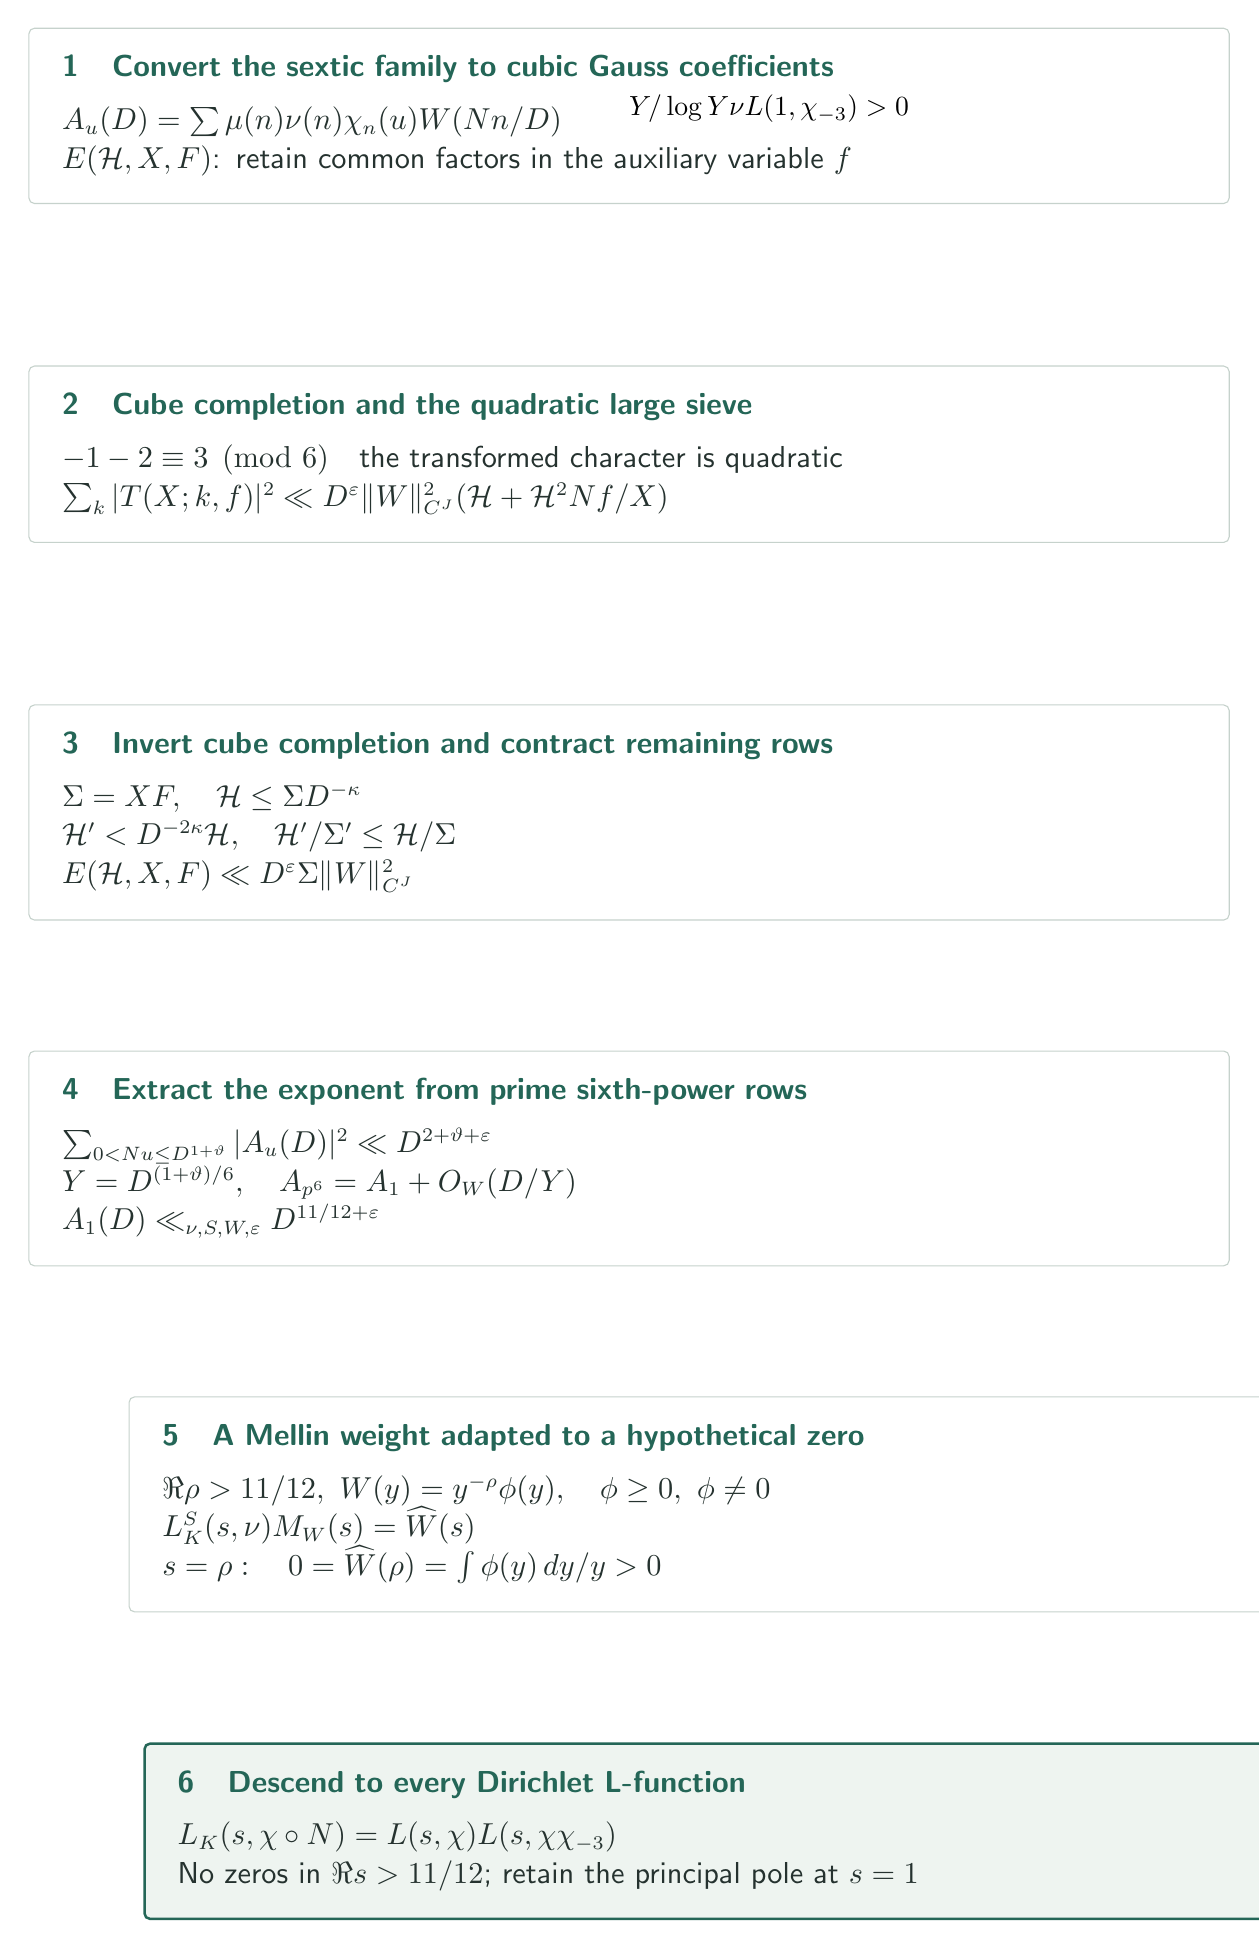
\begin{tikzpicture}
\node[card] (a) {\heading{1}{六次の族を三次Gauss係数へ}{Convert the sextic family to cubic Gauss coefficients}
$A_u(D)=\sum\mu(n)\nu(n)\chi_n(u)W(Nn/D)$\\
$E(\mathcal H,X,F)$: \Tx{共通因子を補助変数 $f$ に保持}{retain common factors in the auxiliary variable $f$}};
\node[card,below=2.05cm of a] (b) {\heading{2}{cube補完と二次large sieve}{Cube completion and the quadratic large sieve}
$-1-2\equiv3\pmod6$\quad\Tx{変換後の指標は二次}{the transformed character is quadratic}\\
$\sum_k|T(X;k,f)|^2\ll D^\varepsilon\|W\|_{C^J}^2(\mathcal H+\mathcal H^2Nf/X)$};
\flow{a}{b}{\Tx{Poisson・係数恒等式の後、固定ray classでtheta変換}{After Poisson and Gauss identities, transform theta in fixed ray classes}\\\Cite{poisson}\quad\Cite{theta}\\\Cite{dr-coefficients}\quad\Cite{gl-input}};
\node[card,below=2.05cm of b] (c) {\heading{3}{cubeを逆変換し、残余の行を縮める}{Invert cube completion and contract remaining rows}
$\Sigma=XF,\quad \mathcal H\le\Sigma D^{-\kappa}$\\
$\mathcal H'<D^{-2\kappa}\mathcal H,\quad\mathcal H'/\Sigma'\le\mathcal H/\Sigma$\\
$E(\mathcal H,X,F)\ll D^\varepsilon\Sigma\|W\|_{C^J}^2$};
\flow{b}{c}{\Tx{短いcube因子を直接評価、長い因子は二度のPoisson変換}{Bound short cube divisors directly; use two Poisson transforms for the rest}\\\Cite{completed}\quad\Cite{iteration}};
\node[card,below=1.65cm of c] (d) {\heading{4}{素イデアルの六乗行から指数を取り出す}{Extract the exponent from prime sixth-power rows}
$\sum_{0<Nu\le D^{1+\vartheta}}|A_u(D)|^2\ll D^{2+\vartheta+\varepsilon}$\\
$Y=D^{(1+\vartheta)/6},\quad A_{p^6}=A_1+O_W(D/Y)$\\
$A_1(D)\ll_{\nu,S,W,\varepsilon}D^{11/12+\varepsilon}$};
\flow{c}{d}{\Tx{元の平均二乗へ戻し、約 $Y/\log Y$ 本の行を平均}{Return to the original mean square and average about $Y/\log Y$ rows}\\\Cite{mobius}};
\node[card,below=1.65cm of d] (e) {\heading{5}{零点に合わせたMellin重みで矛盾}{A Mellin weight adapted to a hypothetical zero}
$\Re\rho>11/12,\ W(y)=y^{-\rho}\phi(y),\quad \phi\ge0,\ \phi\ne0$\\
$L_K^S(s,\nu)M_W(s)=\widehat W(s)$\\
$s=\rho:\quad 0=\widehat W(\rho)=\int\phi(y)\,dy/y>0$};
\flow{d}{e}{\Tx{各指標で正則なMellin積分を得る。定数は $\nu$ に依存してよい}{Obtain a holomorphic Mellin integral for each character; constants may depend on $\nu$}\\\Cite{mellin}};
\node[result,below=1.65cm of e] (f) {\heading{6}{すべてのDirichlet関数へ降下}{Descend to every Dirichlet L-function}
$L_K(s,\chi\circ N)=L(s,\chi)L(s,\chi\chi_{-3})$\\
\Tx{$\Re s>11/12$ に零点なし。$s=1$ の主指標の極を区別}{No zeros in $\Re s>11/12$; retain the principal pole at $s=1$}};
\flow{e}{f}{\Tx{有限Euler因子は非零、$L(1,\chi_{-3})>0$ で極との相殺を除く}{Finite Euler factors are nonzero; $L(1,\chi_{-3})>0$ excludes pole--zero cancellation}\\\Cite{mellin}};

\end{tikzpicture}
\end{document}
